% Options for packages loaded elsewhere
\PassOptionsToPackage{unicode}{hyperref}
\PassOptionsToPackage{hyphens}{url}
%
\documentclass[
]{article}
\usepackage{amsmath,amssymb}
\usepackage{iftex}
\ifPDFTeX
  \usepackage[T1]{fontenc}
  \usepackage[utf8]{inputenc}
  \usepackage{textcomp} % provide euro and other symbols
\else % if luatex or xetex
  \usepackage{unicode-math} % this also loads fontspec
  \defaultfontfeatures{Scale=MatchLowercase}
  \defaultfontfeatures[\rmfamily]{Ligatures=TeX,Scale=1}
\fi
\usepackage{lmodern}
\ifPDFTeX\else
  % xetex/luatex font selection
\fi
% Use upquote if available, for straight quotes in verbatim environments
\IfFileExists{upquote.sty}{\usepackage{upquote}}{}
\IfFileExists{microtype.sty}{% use microtype if available
  \usepackage[]{microtype}
  \UseMicrotypeSet[protrusion]{basicmath} % disable protrusion for tt fonts
}{}
\makeatletter
\@ifundefined{KOMAClassName}{% if non-KOMA class
  \IfFileExists{parskip.sty}{%
    \usepackage{parskip}
  }{% else
    \setlength{\parindent}{0pt}
    \setlength{\parskip}{6pt plus 2pt minus 1pt}}
}{% if KOMA class
  \KOMAoptions{parskip=half}}
\makeatother
\usepackage{xcolor}
\usepackage[margin=1in]{geometry}
\usepackage{color}
\usepackage{fancyvrb}
\newcommand{\VerbBar}{|}
\newcommand{\VERB}{\Verb[commandchars=\\\{\}]}
\DefineVerbatimEnvironment{Highlighting}{Verbatim}{commandchars=\\\{\}}
% Add ',fontsize=\small' for more characters per line
\usepackage{framed}
\definecolor{shadecolor}{RGB}{248,248,248}
\newenvironment{Shaded}{\begin{snugshade}}{\end{snugshade}}
\newcommand{\AlertTok}[1]{\textcolor[rgb]{0.94,0.16,0.16}{#1}}
\newcommand{\AnnotationTok}[1]{\textcolor[rgb]{0.56,0.35,0.01}{\textbf{\textit{#1}}}}
\newcommand{\AttributeTok}[1]{\textcolor[rgb]{0.13,0.29,0.53}{#1}}
\newcommand{\BaseNTok}[1]{\textcolor[rgb]{0.00,0.00,0.81}{#1}}
\newcommand{\BuiltInTok}[1]{#1}
\newcommand{\CharTok}[1]{\textcolor[rgb]{0.31,0.60,0.02}{#1}}
\newcommand{\CommentTok}[1]{\textcolor[rgb]{0.56,0.35,0.01}{\textit{#1}}}
\newcommand{\CommentVarTok}[1]{\textcolor[rgb]{0.56,0.35,0.01}{\textbf{\textit{#1}}}}
\newcommand{\ConstantTok}[1]{\textcolor[rgb]{0.56,0.35,0.01}{#1}}
\newcommand{\ControlFlowTok}[1]{\textcolor[rgb]{0.13,0.29,0.53}{\textbf{#1}}}
\newcommand{\DataTypeTok}[1]{\textcolor[rgb]{0.13,0.29,0.53}{#1}}
\newcommand{\DecValTok}[1]{\textcolor[rgb]{0.00,0.00,0.81}{#1}}
\newcommand{\DocumentationTok}[1]{\textcolor[rgb]{0.56,0.35,0.01}{\textbf{\textit{#1}}}}
\newcommand{\ErrorTok}[1]{\textcolor[rgb]{0.64,0.00,0.00}{\textbf{#1}}}
\newcommand{\ExtensionTok}[1]{#1}
\newcommand{\FloatTok}[1]{\textcolor[rgb]{0.00,0.00,0.81}{#1}}
\newcommand{\FunctionTok}[1]{\textcolor[rgb]{0.13,0.29,0.53}{\textbf{#1}}}
\newcommand{\ImportTok}[1]{#1}
\newcommand{\InformationTok}[1]{\textcolor[rgb]{0.56,0.35,0.01}{\textbf{\textit{#1}}}}
\newcommand{\KeywordTok}[1]{\textcolor[rgb]{0.13,0.29,0.53}{\textbf{#1}}}
\newcommand{\NormalTok}[1]{#1}
\newcommand{\OperatorTok}[1]{\textcolor[rgb]{0.81,0.36,0.00}{\textbf{#1}}}
\newcommand{\OtherTok}[1]{\textcolor[rgb]{0.56,0.35,0.01}{#1}}
\newcommand{\PreprocessorTok}[1]{\textcolor[rgb]{0.56,0.35,0.01}{\textit{#1}}}
\newcommand{\RegionMarkerTok}[1]{#1}
\newcommand{\SpecialCharTok}[1]{\textcolor[rgb]{0.81,0.36,0.00}{\textbf{#1}}}
\newcommand{\SpecialStringTok}[1]{\textcolor[rgb]{0.31,0.60,0.02}{#1}}
\newcommand{\StringTok}[1]{\textcolor[rgb]{0.31,0.60,0.02}{#1}}
\newcommand{\VariableTok}[1]{\textcolor[rgb]{0.00,0.00,0.00}{#1}}
\newcommand{\VerbatimStringTok}[1]{\textcolor[rgb]{0.31,0.60,0.02}{#1}}
\newcommand{\WarningTok}[1]{\textcolor[rgb]{0.56,0.35,0.01}{\textbf{\textit{#1}}}}
\usepackage{graphicx}
\makeatletter
\def\maxwidth{\ifdim\Gin@nat@width>\linewidth\linewidth\else\Gin@nat@width\fi}
\def\maxheight{\ifdim\Gin@nat@height>\textheight\textheight\else\Gin@nat@height\fi}
\makeatother
% Scale images if necessary, so that they will not overflow the page
% margins by default, and it is still possible to overwrite the defaults
% using explicit options in \includegraphics[width, height, ...]{}
\setkeys{Gin}{width=\maxwidth,height=\maxheight,keepaspectratio}
% Set default figure placement to htbp
\makeatletter
\def\fps@figure{htbp}
\makeatother
\setlength{\emergencystretch}{3em} % prevent overfull lines
\providecommand{\tightlist}{%
  \setlength{\itemsep}{0pt}\setlength{\parskip}{0pt}}
\setcounter{secnumdepth}{-\maxdimen} % remove section numbering
\usepackage{booktabs}
\usepackage{caption}
\usepackage{longtable}
\usepackage{colortbl}
\usepackage{array}
\usepackage{anyfontsize}
\usepackage{multirow}
\ifLuaTeX
  \usepackage{selnolig}  % disable illegal ligatures
\fi
\usepackage{bookmark}
\IfFileExists{xurl.sty}{\usepackage{xurl}}{} % add URL line breaks if available
\urlstyle{same}
\hypersetup{
  pdftitle={LAs BEST Project},
  pdfauthor={Justin Coles},
  hidelinks,
  pdfcreator={LaTeX via pandoc}}

\title{LAs BEST Project}
\author{Justin Coles}
\date{2025-06-20}

\begin{document}
\maketitle

<<<<<<< HEAD
\subsection{R Markdown}\label{r-markdown}

This is an R Markdown document. Markdown is a simple formatting syntax
for authoring HTML, PDF, and MS Word documents. For more details on
using R Markdown see \url{http://rmarkdown.rstudio.com}.

When you click the \textbf{Knit} button a document will be generated
that includes both content as well as the output of any embedded R code
chunks within the document. You can embed an R code chunk like this:

\begin{Shaded}
\begin{Highlighting}[]
\FunctionTok{summary}\NormalTok{(cars)}
\end{Highlighting}
\end{Shaded}

\begin{verbatim}
##      speed           dist       
##  Min.   : 4.0   Min.   :  2.00  
##  1st Qu.:12.0   1st Qu.: 26.00  
##  Median :15.0   Median : 36.00  
##  Mean   :15.4   Mean   : 42.98  
##  3rd Qu.:19.0   3rd Qu.: 56.00  
##  Max.   :25.0   Max.   :120.00
\end{verbatim}

\subsection{Including Plots}\label{including-plots}

You can also embed plots, for example:

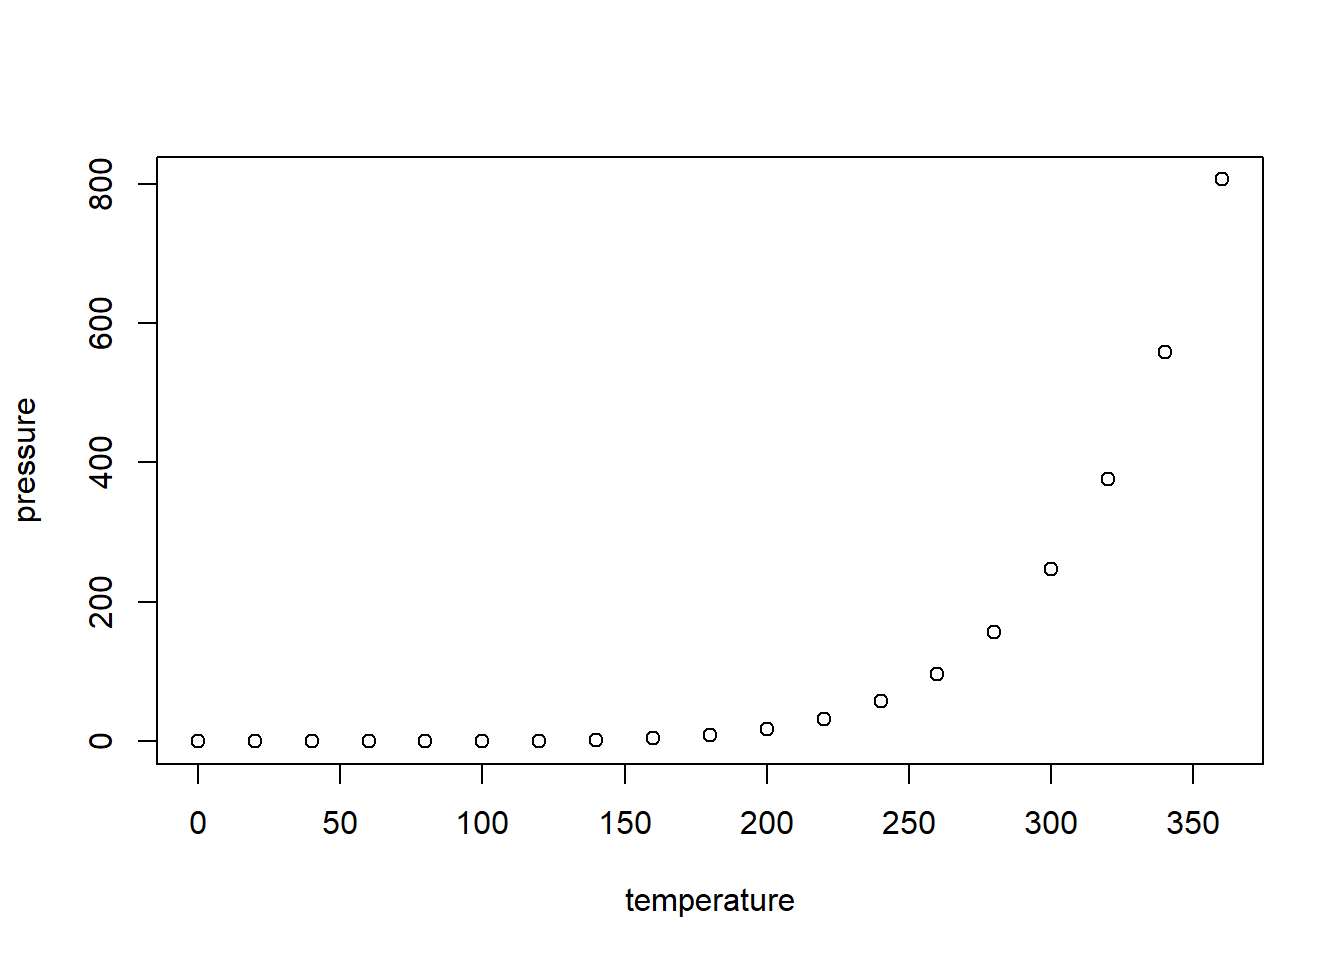
\includegraphics{EDA_EVProj_files/figure-latex/pressure-1.pdf}

=======
>>>>>>> main
Note that the \texttt{echo\ =\ FALSE} parameter was added to the code
chunk to prevent printing of the R code that generated the plot.

\begin{Shaded}
\begin{Highlighting}[]
\FunctionTok{getwd}\NormalTok{()}
\end{Highlighting}
\end{Shaded}

\begin{verbatim}
<<<<<<< HEAD
## [1] "C:/Users/LAs Best/Desktop/EV-Proj_LAsBest"
=======
## [1] "/Users/jessygarcia/LA BEST EV GROUP PROJECT/EV PROJECT"
>>>>>>> main
\end{verbatim}

\begin{Shaded}
\begin{Highlighting}[]
\NormalTok{EV\_data }\OtherTok{\textless{}{-}} \FunctionTok{read.csv}\NormalTok{(}\StringTok{"./Data/data\_ZEV\_asthmaED\_2013\_2022.csv"}\NormalTok{)}
\end{Highlighting}
\end{Shaded}

\begin{Shaded}
\begin{Highlighting}[]
\CommentTok{\#Getting number of EVs per 1000 people}
\NormalTok{EV\_data}\SpecialCharTok{$}\NormalTok{nZEV1000pop }\OtherTok{\textless{}{-}}\NormalTok{ EV\_data}\SpecialCharTok{$}\NormalTok{nZEV}\SpecialCharTok{/}\NormalTok{EV\_data}\SpecialCharTok{$}\NormalTok{pop }\SpecialCharTok{*}\DecValTok{1000}
\CommentTok{\#RoA = Rate of Asthma}
\NormalTok{EV\_data}\SpecialCharTok{$}\NormalTok{log\_AgeAdj\_RoA\_ED\_Visit\_Rate }\OtherTok{\textless{}{-}} \FunctionTok{log}\NormalTok{(EV\_data}\SpecialCharTok{$}\NormalTok{Age\_Adjusted\_Rate\_of\_Asthma\_ED\_Visit\_Rate)}
\CommentTok{\#Getting LN to help create better plots }
\end{Highlighting}
\end{Shaded}

\begin{Shaded}
\begin{Highlighting}[]
\CommentTok{\#Summary Stats by all years}
\NormalTok{summary\_stats\_allyrs }\OtherTok{\textless{}{-}} \FunctionTok{c}\NormalTok{(}
\FunctionTok{summary}\NormalTok{(EV\_data}\SpecialCharTok{$}\NormalTok{Age\_Adjusted\_Rate\_of\_Asthma\_ED\_Visit\_Rate),}
\AttributeTok{SD=}\FunctionTok{sd}\NormalTok{(EV\_data}\SpecialCharTok{$}\NormalTok{Age\_Adjusted\_Rate\_of\_Asthma\_ED\_Visit\_Rate))}
<<<<<<< HEAD
=======

\NormalTok{summary\_stats\_allyrs}
\end{Highlighting}
\end{Shaded}

\begin{verbatim}
##      Min.   1st Qu.    Median      Mean   3rd Qu.      Max.        SD 
##   2.90000  22.50000  34.90000  41.90312  52.60000 669.30000  28.98692
\end{verbatim}

\begin{Shaded}
\begin{Highlighting}[]
>>>>>>> main
\CommentTok{\#mean(41.90) {-}{-}\textgreater{} \#there are about 41.90 visits to ED per 10,000ppl}
\CommentTok{\#Sd(28.98) {-}{-}\textgreater{} there is huge variance between zip codes and ppl in ED }
\end{Highlighting}
\end{Shaded}

\begin{Shaded}
\begin{Highlighting}[]
\CommentTok{\#Summary Stats by each years}
\FunctionTok{cat}\NormalTok{(}\StringTok{"Summary Statistics of Asthma ED Visit Rates by Year:}\SpecialCharTok{\textbackslash{}n}\StringTok{"}\NormalTok{)}
\end{Highlighting}
\end{Shaded}

\begin{verbatim}
## Summary Statistics of Asthma ED Visit Rates by Year:
\end{verbatim}

\begin{Shaded}
\begin{Highlighting}[]
\FunctionTok{print}\NormalTok{(}\FunctionTok{tapply}\NormalTok{(EV\_data}\SpecialCharTok{$}\NormalTok{Age\_Adjusted\_Rate\_of\_Asthma\_ED\_Visit\_Rate, EV\_data}\SpecialCharTok{$}\NormalTok{yr, summary, }\AttributeTok{na.rm =} \ConstantTok{TRUE}\NormalTok{))}
\end{Highlighting}
\end{Shaded}

\begin{verbatim}
## $`2013`
##    Min. 1st Qu.  Median    Mean 3rd Qu.    Max. 
##    7.60   28.20   42.85   49.51   60.98  278.10 
## 
## $`2014`
##    Min. 1st Qu.  Median    Mean 3rd Qu.    Max. 
##    7.00   28.00   43.75   49.69   61.42  252.20 
## 
## $`2015`
##    Min. 1st Qu.  Median    Mean 3rd Qu.    Max. 
##    6.80   29.40   45.20   51.45   64.60  323.40 
## 
## $`2016`
##    Min. 1st Qu.  Median    Mean 3rd Qu.    Max. 
##    5.80   26.50   39.10   46.30   58.05  358.90 
## 
## $`2017`
##    Min. 1st Qu.  Median    Mean 3rd Qu.    Max. 
##    5.80   27.30   41.40   48.63   59.30  669.30 
## 
## $`2018`
##    Min. 1st Qu.  Median    Mean 3rd Qu.    Max. 
##    6.50   23.95   37.20   43.27   52.75  311.30 
## 
## $`2019`
##    Min. 1st Qu.  Median    Mean 3rd Qu.    Max. 
##    6.80   23.90   37.40   43.03   53.17  350.40 
## 
## $`2020`
##    Min. 1st Qu.  Median    Mean 3rd Qu.    Max. 
##    2.90   14.40   21.90   25.63   31.60  210.30 
## 
## $`2021`
##    Min. 1st Qu.  Median    Mean 3rd Qu.    Max. 
##    3.20   14.60   21.20   25.38   30.90  172.60 
## 
## $`2022`
##    Min. 1st Qu.  Median    Mean 3rd Qu.    Max. 
##    5.70   20.00   28.90   32.57   39.90  204.80
\end{verbatim}

\begin{Shaded}
\begin{Highlighting}[]
\FunctionTok{cat}\NormalTok{(}\StringTok{"}\SpecialCharTok{\textbackslash{}n}\StringTok{Standard Deviation by Year:}\SpecialCharTok{\textbackslash{}n}\StringTok{"}\NormalTok{)}
\end{Highlighting}
\end{Shaded}

\begin{verbatim}
## 
## Standard Deviation by Year:
\end{verbatim}

\begin{Shaded}
\begin{Highlighting}[]
\FunctionTok{print}\NormalTok{(}\FunctionTok{tapply}\NormalTok{(EV\_data}\SpecialCharTok{$}\NormalTok{Age\_Adjusted\_Rate\_of\_Asthma\_ED\_Visit\_Rate , EV\_data}\SpecialCharTok{$}\NormalTok{yr , sd, }\AttributeTok{na.rm =} \ConstantTok{TRUE}\NormalTok{))}
\end{Highlighting}
\end{Shaded}

\begin{verbatim}
##     2013     2014     2015     2016     2017     2018     2019     2020 
## 30.54874 30.64675 31.89268 29.60630 34.83508 28.00668 27.49992 17.14249 
##     2021     2022 
## 16.86820 18.16043
\end{verbatim}

\begin{Shaded}
\begin{Highlighting}[]
\FunctionTok{tapply}\NormalTok{(EV\_data}\SpecialCharTok{$}\NormalTok{nZEV, EV\_data}\SpecialCharTok{$}\NormalTok{yr, summary, }\AttributeTok{na.rm =} \ConstantTok{TRUE}\NormalTok{) }
\end{Highlighting}
\end{Shaded}

\begin{verbatim}
## $`2013`
##    Min. 1st Qu.  Median    Mean 3rd Qu.    Max. 
##    0.00    5.75   21.00   42.55   55.00  489.00 
## 
## $`2014`
##    Min. 1st Qu.  Median    Mean 3rd Qu.    Max. 
##    0.00   14.00   48.00   88.41  119.00 1031.00 
## 
## $`2015`
##    Min. 1st Qu.  Median    Mean 3rd Qu.    Max. 
##     0.0    21.0    76.0   134.5   182.0  1612.0 
## 
## $`2016`
##    Min. 1st Qu.  Median    Mean 3rd Qu.    Max. 
##     0.0    33.0   111.0   187.9   258.0  2061.0 
## 
## $`2017`
##    Min. 1st Qu.  Median    Mean 3rd Qu.    Max. 
##     0.0    51.0   165.0   264.8   368.2  2627.0 
## 
## $`2018`
##    Min. 1st Qu.  Median    Mean 3rd Qu.    Max. 
##     0.0    74.5   236.0   373.8   520.0  3592.0 
## 
## $`2019`
##    Min. 1st Qu.  Median    Mean 3rd Qu.    Max. 
##     0.0   103.0   306.5   466.1   647.0  4153.0 
## 
## $`2020`
##    Min. 1st Qu.  Median    Mean 3rd Qu.    Max. 
##     1.0   146.0   381.0   544.1   764.0  4180.0 
## 
## $`2021`
##    Min. 1st Qu.  Median    Mean 3rd Qu.    Max. 
##     1.0   212.5   534.0   716.8  1021.5  4743.0 
## 
## $`2022`
##    Min. 1st Qu.  Median    Mean 3rd Qu.    Max. 
##     1.0   262.0   701.0   931.4  1317.0  6913.0
\end{verbatim}

\begin{Shaded}
\begin{Highlighting}[]
\FunctionTok{tapply}\NormalTok{(EV\_data}\SpecialCharTok{$}\NormalTok{nZEV, EV\_data}\SpecialCharTok{$}\NormalTok{yr, sd,      }\AttributeTok{na.rm =} \ConstantTok{TRUE}\NormalTok{)}
\end{Highlighting}
\end{Shaded}

\begin{verbatim}
##      2013      2014      2015      2016      2017      2018      2019      2020 
##  59.14079 113.51789 170.70389 231.28399 309.07842 427.45095 515.11476 562.29624 
##      2021      2022 
## 693.50239 915.31649
\end{verbatim}

\begin{Shaded}
\begin{Highlighting}[]
\FunctionTok{tapply}\NormalTok{(EV\_data}\SpecialCharTok{$}\NormalTok{nZEV1000pop , EV\_data}\SpecialCharTok{$}\NormalTok{yr, summary, }\AttributeTok{na.rm =} \ConstantTok{TRUE}\NormalTok{) }
\end{Highlighting}
\end{Shaded}

\begin{verbatim}
## $`2013`
##    Min. 1st Qu.  Median    Mean 3rd Qu.    Max. 
##  0.0000  0.2376  0.6575  1.4236  1.8277 19.6846 
## 
## $`2014`
##    Min. 1st Qu.  Median    Mean 3rd Qu.    Max. 
##  0.0000  0.5902  1.5740  2.8940  3.9506 25.6807 
## 
## $`2015`
##    Min. 1st Qu.  Median    Mean 3rd Qu.    Max. 
##  0.0000  0.8642  2.5219  4.4183  5.9540 38.9570 
## 
## $`2016`
##    Min. 1st Qu.  Median    Mean 3rd Qu.    Max. 
##   0.000   1.347   3.593   6.087   8.174  51.788 
## 
## $`2017`
##    Min. 1st Qu.  Median    Mean 3rd Qu.    Max. 
##   0.000   2.049   5.366   8.668  12.182  67.299 
## 
## $`2018`
##    Min. 1st Qu.  Median    Mean 3rd Qu.    Max. 
##   0.000   2.965   7.768  12.103  16.944  91.312 
## 
## $`2019`
##    Min. 1st Qu.  Median    Mean 3rd Qu.    Max. 
##   0.000   3.941   9.961  14.721  20.482 101.309 
## 
## $`2020`
##    Min. 1st Qu.  Median    Mean 3rd Qu.    Max. 
##   0.190   4.868  11.445  15.982  22.439  98.538 
## 
## $`2021`
##    Min. 1st Qu.  Median    Mean 3rd Qu.    Max. 
##   0.386   7.141  15.822  20.928  29.400 135.695 
## 
## $`2022`
##    Min. 1st Qu.  Median    Mean 3rd Qu.    Max. 
##   0.386   9.738  21.961  28.464  39.254 245.957
\end{verbatim}

\begin{Shaded}
\begin{Highlighting}[]
\FunctionTok{tapply}\NormalTok{(EV\_data}\SpecialCharTok{$}\NormalTok{nZEV1000pop , EV\_data}\SpecialCharTok{$}\NormalTok{yr, sd,      }\AttributeTok{na.rm =} \ConstantTok{TRUE}\NormalTok{)}
\end{Highlighting}
\end{Shaded}

\begin{verbatim}
##      2013      2014      2015      2016      2017      2018      2019      2020 
##  2.042576  3.587522  5.352172  7.063109  9.509201 12.952706 14.702309 14.870094 
##      2021      2022 
## 18.269126 25.380152
\end{verbatim}

\begin{Shaded}
\begin{Highlighting}[]
\FunctionTok{tapply}\NormalTok{(EV\_data}\SpecialCharTok{$}\NormalTok{pop , EV\_data}\SpecialCharTok{$}\NormalTok{yr, summary, }\AttributeTok{na.rm =} \ConstantTok{TRUE}\NormalTok{) }
\end{Highlighting}
\end{Shaded}

\begin{verbatim}
## $`2013`
##    Min. 1st Qu.  Median    Mean 3rd Qu.    Max. 
##     702   16580   30951   33023   45452  111165 
## 
## $`2014`
##    Min. 1st Qu.  Median    Mean 3rd Qu.    Max. 
##    1281   16580   30951   33013   45452  111165 
## 
## $`2015`
##    Min. 1st Qu.  Median    Mean 3rd Qu.    Max. 
<<<<<<< HEAD
##     702   16258   30611   32681   45231  111165 
## 
## $`2016`
##    Min. 1st Qu.  Median    Mean 3rd Qu.    Max. 
##    1246   16413   30787   32931   45440  111165 
=======
##     702   16258   30611   32681   45230  111165 
## 
## $`2016`
##    Min. 1st Qu.  Median    Mean 3rd Qu.    Max. 
##    1246   16412   30787   32931   45440  111165 
>>>>>>> main
## 
## $`2017`
##    Min. 1st Qu.  Median    Mean 3rd Qu.    Max. 
##    1159   16270   30714   32709   45163  111165 
## 
## $`2018`
##    Min. 1st Qu.  Median    Mean 3rd Qu.    Max. 
<<<<<<< HEAD
##    1246   16644   31000   33052   45461  111165 
## 
## $`2019`
##    Min. 1st Qu.  Median    Mean 3rd Qu.    Max. 
##    1289   16852   31179   33232   45775  111165 
=======
##    1246   16644   31000   33052   45460  111165 
## 
## $`2019`
##    Min. 1st Qu.  Median    Mean 3rd Qu.    Max. 
##    1289   16852   31178   33232   45775  111165 
>>>>>>> main
## 
## $`2020`
##    Min. 1st Qu.  Median    Mean 3rd Qu.    Max. 
##    1615   20666   33234   35487   47081  111165 
## 
## $`2021`
##    Min. 1st Qu.  Median    Mean 3rd Qu.    Max. 
##    1615   20670   33234   35491   47096  111165 
## 
## $`2022`
##    Min. 1st Qu.  Median    Mean 3rd Qu.    Max. 
##    1462   18591   31936   34067   46241  111165
\end{verbatim}

\begin{Shaded}
\begin{Highlighting}[]
\FunctionTok{tapply}\NormalTok{(EV\_data}\SpecialCharTok{$}\NormalTok{pop , EV\_data}\SpecialCharTok{$}\NormalTok{yr, sd,      }\AttributeTok{na.rm =} \ConstantTok{TRUE}\NormalTok{)}
\end{Highlighting}
\end{Shaded}

\begin{verbatim}
##     2013     2014     2015     2016     2017     2018     2019     2020 
## 20795.99 20803.96 20943.63 20839.85 20918.00 20782.13 20753.63 20159.38 
##     2021     2022 
## 20182.61 20547.30
\end{verbatim}

\begin{Shaded}
\begin{Highlighting}[]
\FunctionTok{tapply}\NormalTok{(EV\_data}\SpecialCharTok{$}\NormalTok{percPoverty , EV\_data}\SpecialCharTok{$}\NormalTok{yr, summary, }\AttributeTok{na.rm =} \ConstantTok{TRUE}\NormalTok{) }
\end{Highlighting}
\end{Shaded}

\begin{verbatim}
## $`2013`
##    Min. 1st Qu.  Median    Mean 3rd Qu.    Max. 
##    0.00    7.40   11.45   13.64   18.02   56.70 
## 
## $`2014`
##    Min. 1st Qu.  Median    Mean 3rd Qu.    Max. 
##    0.00    7.40   11.45   13.68   17.93   56.70 
## 
## $`2015`
##    Min. 1st Qu.  Median    Mean 3rd Qu.    Max. 
##    0.00    7.40   11.50   13.74   18.10   56.70 
## 
## $`2016`
##    Min. 1st Qu.  Median    Mean 3rd Qu.    Max. 
##    0.00    7.40   11.50   13.71   18.10   56.70 
## 
## $`2017`
##    Min. 1st Qu.  Median    Mean 3rd Qu.    Max. 
##    0.00    7.40   11.50   13.69   18.10   49.40 
## 
## $`2018`
##    Min. 1st Qu.  Median    Mean 3rd Qu.    Max. 
##    0.00    7.40   11.50   13.67   18.05   49.40 
## 
## $`2019`
##    Min. 1st Qu.  Median    Mean 3rd Qu.    Max. 
##    0.00    7.40   11.50   13.78   18.18   56.70 
## 
## $`2020`
##    Min. 1st Qu.  Median    Mean 3rd Qu.    Max. 
##     0.0     7.5    11.6    13.8    18.2    49.4 
## 
## $`2021`
##    Min. 1st Qu.  Median    Mean 3rd Qu.    Max. 
##     0.0     7.5    11.6    13.8    18.2    56.7 
## 
## $`2022`
##    Min. 1st Qu.  Median    Mean 3rd Qu.    Max. 
##     0.0     7.5    11.6    13.7    18.1    49.4
\end{verbatim}

\begin{Shaded}
\begin{Highlighting}[]
\FunctionTok{tapply}\NormalTok{(EV\_data}\SpecialCharTok{$}\NormalTok{percPoverty , EV\_data}\SpecialCharTok{$}\NormalTok{yr, sd,      }\AttributeTok{na.rm =} \ConstantTok{TRUE}\NormalTok{)}
\end{Highlighting}
\end{Shaded}

\begin{verbatim}
##     2013     2014     2015     2016     2017     2018     2019     2020 
## 8.515461 8.595512 8.556429 8.541994 8.505724 8.515091 8.597460 8.345641 
##     2021     2022 
## 8.366060 8.360286
\end{verbatim}

\begin{Shaded}
\begin{Highlighting}[]
\FunctionTok{tapply}\NormalTok{(EV\_data}\SpecialCharTok{$}\NormalTok{HHincomeMedian , EV\_data}\SpecialCharTok{$}\NormalTok{yr, summary, }\AttributeTok{na.rm =} \ConstantTok{TRUE}\NormalTok{) }
\end{Highlighting}
\end{Shaded}

\begin{verbatim}
## $`2013`
##    Min. 1st Qu.  Median    Mean 3rd Qu.    Max. 
##   14822   53904   73169   79830   97399  250000 
## 
## $`2014`
##    Min. 1st Qu.  Median    Mean 3rd Qu.    Max. 
##   14822   53927   73169   79676   97690  250000 
## 
## $`2015`
##    Min. 1st Qu.  Median    Mean 3rd Qu.    Max. 
##   14822   53647   72995   79531   97054  250000 
## 
## $`2016`
##    Min. 1st Qu.  Median    Mean 3rd Qu.    Max. 
<<<<<<< HEAD
##   14822   54039   73093   79732   97451  250000 
## 
## $`2017`
##    Min. 1st Qu.  Median    Mean 3rd Qu.    Max. 
##   14822   53927   73063   79771   97583  250000 
## 
## $`2018`
##    Min. 1st Qu.  Median    Mean 3rd Qu.    Max. 
##   14822   54039   73151   79986   97918  250000 
## 
## $`2019`
##    Min. 1st Qu.  Median    Mean 3rd Qu.    Max. 
##   14822   53804   73093   79391   97117  237841 
=======
##   14822   54038   73093   79732   97450  250000 
## 
## $`2017`
##    Min. 1st Qu.  Median    Mean 3rd Qu.    Max. 
##   14822   53927   73062   79771   97583  250000 
## 
## $`2018`
##    Min. 1st Qu.  Median    Mean 3rd Qu.    Max. 
##   14822   54038   73151   79986   97918  250000 
## 
## $`2019`
##    Min. 1st Qu.  Median    Mean 3rd Qu.    Max. 
##   14822   53804   73093   79391   97116  237841 
>>>>>>> main
## 
## $`2020`
##    Min. 1st Qu.  Median    Mean 3rd Qu.    Max. 
##   14822   54167   72926   78597   96085  222930 
## 
## $`2021`
##    Min. 1st Qu.  Median    Mean 3rd Qu.    Max. 
<<<<<<< HEAD
##   14822   54139   72778   78621   95987  222930 
=======
##   14822   54138   72778   78621   95987  222930 
>>>>>>> main
## 
## $`2022`
##    Min. 1st Qu.  Median    Mean 3rd Qu.    Max. 
##   14822   54110   73093   79370   97179  250000
\end{verbatim}

\begin{Shaded}
\begin{Highlighting}[]
\FunctionTok{tapply}\NormalTok{(EV\_data}\SpecialCharTok{$}\NormalTok{HHincomeMedian , EV\_data}\SpecialCharTok{$}\NormalTok{yr, sd,      }\AttributeTok{na.rm =} \ConstantTok{TRUE}\NormalTok{)}
\end{Highlighting}
\end{Shaded}

\begin{verbatim}
##     2013     2014     2015     2016     2017     2018     2019     2020 
## 34407.73 33890.76 34193.40 34167.45 34396.12 34483.68 33634.67 32015.01 
##     2021     2022 
## 32190.08 33185.61
\end{verbatim}

\begin{Shaded}
\begin{Highlighting}[]
\FunctionTok{tapply}\NormalTok{(EV\_data}\SpecialCharTok{$}\NormalTok{HHincomeMean , EV\_data}\SpecialCharTok{$}\NormalTok{yr, summary, }\AttributeTok{na.rm =} \ConstantTok{TRUE}\NormalTok{) }
\end{Highlighting}
\end{Shaded}

\begin{verbatim}
## $`2013`
##    Min. 1st Qu.  Median    Mean 3rd Qu.    Max. 
<<<<<<< HEAD
##   28973   72494   93745  104685  126755  347939 
## 
## $`2014`
##    Min. 1st Qu.  Median    Mean 3rd Qu.    Max. 
##   28973   72676   93830  104482  126755  344838 
## 
## $`2015`
##    Min. 1st Qu.  Median    Mean 3rd Qu.    Max. 
##   28973   72082   93755  104552  126601  347939 
=======
##   28973   72494   93744  104685  126754  347939 
## 
## $`2014`
##    Min. 1st Qu.  Median    Mean 3rd Qu.    Max. 
##   28973   72676   93830  104482  126754  344838 
## 
## $`2015`
##    Min. 1st Qu.  Median    Mean 3rd Qu.    Max. 
##   28973   72082   93755  104552  126600  347939 
>>>>>>> main
## 
## $`2016`
##    Min. 1st Qu.  Median    Mean 3rd Qu.    Max. 
##   28973   72595   93734  104509  126762  347939 
## 
## $`2017`
##    Min. 1st Qu.  Median    Mean 3rd Qu.    Max. 
<<<<<<< HEAD
##   28973   72386   93723  104548  126755  347939 
=======
##   28973   72386   93723  104548  126754  347939 
>>>>>>> main
## 
## $`2018`
##    Min. 1st Qu.  Median    Mean 3rd Qu.    Max. 
##   28973   72595   93904  105042  126809  347939 
## 
## $`2019`
##    Min. 1st Qu.  Median    Mean 3rd Qu.    Max. 
<<<<<<< HEAD
##   28973   71918   93745  103864  125516  347939 
=======
##   28973   71918   93744  103864  125516  347939 
>>>>>>> main
## 
## $`2020`
##    Min. 1st Qu.  Median    Mean 3rd Qu.    Max. 
##   28973   72298   93416  102113  124232  312860 
## 
## $`2021`
##    Min. 1st Qu.  Median    Mean 3rd Qu.    Max. 
<<<<<<< HEAD
##   28973   72357   93363  102219  124080  325745 
=======
##   28973   72356   93363  102219  124080  325745 
>>>>>>> main
## 
## $`2022`
##    Min. 1st Qu.  Median    Mean 3rd Qu.    Max. 
##   28973   72520   93973  103515  125416  344838
\end{verbatim}

\begin{Shaded}
\begin{Highlighting}[]
\FunctionTok{tapply}\NormalTok{(EV\_data}\SpecialCharTok{$}\NormalTok{HHincomeMean , EV\_data}\SpecialCharTok{$}\NormalTok{yr, sd,      }\AttributeTok{na.rm =} \ConstantTok{TRUE}\NormalTok{)}
\end{Highlighting}
\end{Shaded}

\begin{verbatim}
##     2013     2014     2015     2016     2017     2018     2019     2020 
## 46741.51 45815.85 46667.70 46040.89 46476.86 47218.44 45045.16 41329.46 
##     2021     2022 
## 41785.86 43532.31
\end{verbatim}

\begin{Shaded}
\begin{Highlighting}[]
\FunctionTok{tapply}\NormalTok{(EV\_data}\SpecialCharTok{$}\NormalTok{EDUCpercHSplus , EV\_data}\SpecialCharTok{$}\NormalTok{yr, summary, }\AttributeTok{na.rm =} \ConstantTok{TRUE}\NormalTok{) }
\end{Highlighting}
\end{Shaded}

\begin{verbatim}
## $`2013`
##    Min. 1st Qu.  Median    Mean 3rd Qu.    Max. 
##   28.90   77.20   87.70   83.57   93.40   99.40 
## 
## $`2014`
##    Min. 1st Qu.  Median    Mean 3rd Qu.    Max. 
##   28.90   77.28   87.70   83.63   93.40   99.70 
## 
## $`2015`
##    Min. 1st Qu.  Median    Mean 3rd Qu.    Max. 
##   28.90   77.15   87.70   83.51   93.35   99.70 
## 
## $`2016`
##    Min. 1st Qu.  Median    Mean 3rd Qu.    Max. 
##   28.90   77.10   87.50   83.45   93.30   99.20 
## 
## $`2017`
##    Min. 1st Qu.  Median    Mean 3rd Qu.    Max. 
##   28.90   77.28   87.70   83.64   93.40   99.70 
## 
## $`2018`
##    Min. 1st Qu.  Median    Mean 3rd Qu.    Max. 
##   28.90   77.25   87.70   83.61   93.40   99.70 
## 
## $`2019`
##    Min. 1st Qu.  Median    Mean 3rd Qu.    Max. 
##   28.90   77.10   87.45   83.41   93.30   99.70 
## 
## $`2020`
##    Min. 1st Qu.  Median    Mean 3rd Qu.    Max. 
##   28.90   76.70   86.80   82.96   92.90   98.70 
## 
## $`2021`
##    Min. 1st Qu.  Median    Mean 3rd Qu.    Max. 
##   28.90   76.70   86.70   82.95   92.95   99.40 
## 
## $`2022`
##    Min. 1st Qu.  Median    Mean 3rd Qu.    Max. 
##   28.90   77.10   87.20   83.35   93.10   99.40
\end{verbatim}

\begin{Shaded}
\begin{Highlighting}[]
\FunctionTok{tapply}\NormalTok{(EV\_data}\SpecialCharTok{$}\NormalTok{EDUCpercHSplus , EV\_data}\SpecialCharTok{$}\NormalTok{yr, sd,      }\AttributeTok{na.rm =} \ConstantTok{TRUE}\NormalTok{)}
\end{Highlighting}
\end{Shaded}

\begin{verbatim}
##     2013     2014     2015     2016     2017     2018     2019     2020 
## 13.10635 13.08708 13.13854 13.11851 13.01871 13.03838 13.11825 13.00763 
##     2021     2022 
## 13.04708 12.92799
\end{verbatim}

\begin{Shaded}
\begin{Highlighting}[]
\FunctionTok{tapply}\NormalTok{(EV\_data}\SpecialCharTok{$}\NormalTok{EDUCpercBAplus , EV\_data}\SpecialCharTok{$}\NormalTok{yr, summary, }\AttributeTok{na.rm =} \ConstantTok{TRUE}\NormalTok{) }
\end{Highlighting}
\end{Shaded}

\begin{verbatim}
## $`2013`
##    Min. 1st Qu.  Median    Mean 3rd Qu.    Max. 
##    1.10   17.30   29.95   33.53   47.42   87.10 
## 
## $`2014`
##    Min. 1st Qu.  Median    Mean 3rd Qu.    Max. 
##    1.10   17.20   30.10   33.55   47.42   87.10 
## 
## $`2015`
##    Min. 1st Qu.  Median    Mean 3rd Qu.    Max. 
##    1.10   17.10   30.00   33.48   47.35   86.80 
## 
## $`2016`
##    Min. 1st Qu.  Median    Mean 3rd Qu.    Max. 
##    1.10   17.25   29.80   33.40   47.25   87.10 
## 
## $`2017`
##    Min. 1st Qu.  Median    Mean 3rd Qu.    Max. 
##    1.10   17.38   29.85   33.55   47.50   87.10 
## 
## $`2018`
##    Min. 1st Qu.  Median    Mean 3rd Qu.    Max. 
##    1.10   17.35   29.90   33.66   47.50   87.10 
## 
## $`2019`
##    Min. 1st Qu.  Median    Mean 3rd Qu.    Max. 
##    1.10   17.12   29.80   33.33   47.27   86.80 
## 
## $`2020`
##    Min. 1st Qu.  Median    Mean 3rd Qu.    Max. 
##    1.10   17.20   29.60   32.77   46.40   82.60 
## 
## $`2021`
##    Min. 1st Qu.  Median    Mean 3rd Qu.    Max. 
##    1.10   17.20   29.50   32.83   46.70   83.00 
## 
## $`2022`
##    Min. 1st Qu.  Median    Mean 3rd Qu.    Max. 
##    1.10   17.30   29.90   33.25   46.70   85.70
\end{verbatim}

\begin{Shaded}
\begin{Highlighting}[]
\FunctionTok{tapply}\NormalTok{(EV\_data}\SpecialCharTok{$}\NormalTok{EDUCpercBAplus , EV\_data}\SpecialCharTok{$}\NormalTok{yr, sd,      }\AttributeTok{na.rm =} \ConstantTok{TRUE}\NormalTok{)}
\end{Highlighting}
\end{Shaded}

\begin{verbatim}
##     2013     2014     2015     2016     2017     2018     2019     2020 
## 19.89249 19.94024 19.96842 19.87392 19.94324 20.08068 19.86764 19.04289 
##     2021     2022 
## 19.13299 19.48771
\end{verbatim}

\begin{Shaded}
\begin{Highlighting}[]
\CommentTok{\#New dataset with just the variables of interest for Corr. Matrix}

\FunctionTok{library}\NormalTok{(corrplot)}
\end{Highlighting}
\end{Shaded}

\begin{verbatim}
<<<<<<< HEAD
## Warning: package 'corrplot' was built under R version 4.4.3
\end{verbatim}

\begin{verbatim}
=======
>>>>>>> main
## corrplot 0.95 loaded
\end{verbatim}

\begin{Shaded}
\begin{Highlighting}[]
\NormalTok{corr\_EV\_data\_vars }\OtherTok{\textless{}{-}}\NormalTok{ EV\_data[, }\FunctionTok{c}\NormalTok{(}
  \StringTok{"nZEV"}\NormalTok{,                      }\CommentTok{\# number of electric vehicles}
<<<<<<< HEAD
  \StringTok{"nZEV1000pop"}\NormalTok{,              }\CommentTok{\# EVs per 1000 people}
  \StringTok{"pop"}\NormalTok{,                      }\CommentTok{\# population}
  \StringTok{"Age\_Adjusted\_Rate\_of\_Asthma\_ED\_Visit\_Rate"}\NormalTok{,  }\CommentTok{\# asthma outcomlie}
=======
  \StringTok{"nZEV1000pop"}\NormalTok{,              }\CommentTok{\# EVs per 1000 people (you created this)}
  \StringTok{"pop"}\NormalTok{,                      }\CommentTok{\# population}
  \StringTok{"Age\_Adjusted\_Rate\_of\_Asthma\_ED\_Visit\_Rate"}\NormalTok{,  }\CommentTok{\# asthma outcome}
>>>>>>> main
  \StringTok{"percPoverty"}\NormalTok{,              }\CommentTok{\# poverty \%}
  \StringTok{"HHincomeMedian"}\NormalTok{,           }\CommentTok{\# median income}
  \StringTok{"HHincomeMean"}\NormalTok{,             }\CommentTok{\# mean income}
  \StringTok{"EDUCpercHSplus"}\NormalTok{,           }\CommentTok{\# \% with high school education or higher}
  \StringTok{"EDUCpercBAplus"}            \CommentTok{\# \% with bachelor’s degree or higher}
\NormalTok{)]}

\NormalTok{corr\_EV\_data\_matrix }\OtherTok{\textless{}{-}} \FunctionTok{cor}\NormalTok{(corr\_EV\_data\_vars, }\AttributeTok{use =} \StringTok{"complete.obs"}\NormalTok{)}
\FunctionTok{print}\NormalTok{(corr\_EV\_data\_matrix)}
\end{Highlighting}
\end{Shaded}

\begin{verbatim}
##                                                 nZEV nZEV1000pop         pop
## nZEV                                       1.0000000  0.82739968  0.26510142
## nZEV1000pop                                0.8273997  1.00000000 -0.04152062
## pop                                        0.2651014 -0.04152062  1.00000000
## Age_Adjusted_Rate_of_Asthma_ED_Visit_Rate -0.3908522 -0.40111769 -0.04671280
## percPoverty                               -0.3481436 -0.37907673 -0.04634126
## HHincomeMedian                             0.4953929  0.57475848  0.01077475
## HHincomeMean                               0.4883625  0.60065490 -0.03456219
## EDUCpercHSplus                             0.3231912  0.39995856 -0.13220974
## EDUCpercBAplus                             0.4813832  0.58683326 -0.06569007
##                                           Age_Adjusted_Rate_of_Asthma_ED_Visit_Rate
## nZEV                                                                     -0.3908522
## nZEV1000pop                                                              -0.4011177
## pop                                                                      -0.0467128
## Age_Adjusted_Rate_of_Asthma_ED_Visit_Rate                                 1.0000000
## percPoverty                                                               0.5008629
## HHincomeMedian                                                           -0.4965716
## HHincomeMean                                                             -0.4891219
## EDUCpercHSplus                                                           -0.3656324
## EDUCpercBAplus                                                           -0.4740336
##                                           percPoverty HHincomeMedian
## nZEV                                      -0.34814358     0.49539288
## nZEV1000pop                               -0.37907673     0.57475848
## pop                                       -0.04634126     0.01077475
## Age_Adjusted_Rate_of_Asthma_ED_Visit_Rate  0.50086288    -0.49657156
## percPoverty                                1.00000000    -0.75584799
## HHincomeMedian                            -0.75584799     1.00000000
## HHincomeMean                              -0.68585072     0.96034650
## EDUCpercHSplus                            -0.67150251     0.63134316
## EDUCpercBAplus                            -0.56630830     0.79325673
##                                           HHincomeMean EDUCpercHSplus
## nZEV                                        0.48836247      0.3231912
## nZEV1000pop                                 0.60065490      0.3999586
## pop                                        -0.03456219     -0.1322097
## Age_Adjusted_Rate_of_Asthma_ED_Visit_Rate  -0.48912191     -0.3656324
## percPoverty                                -0.68585072     -0.6715025
## HHincomeMedian                              0.96034650      0.6313432
## HHincomeMean                                1.00000000      0.6298838
## EDUCpercHSplus                              0.62988382      1.0000000
## EDUCpercBAplus                              0.84432010      0.7558573
##                                           EDUCpercBAplus
## nZEV                                          0.48138322
## nZEV1000pop                                   0.58683326
## pop                                          -0.06569007
## Age_Adjusted_Rate_of_Asthma_ED_Visit_Rate    -0.47403364
## percPoverty                                  -0.56630830
## HHincomeMedian                                0.79325673
## HHincomeMean                                  0.84432010
## EDUCpercHSplus                                0.75585726
## EDUCpercBAplus                                1.00000000
\end{verbatim}

\begin{Shaded}
\begin{Highlighting}[]
<<<<<<< HEAD
\FunctionTok{library}\NormalTok{(ggplot2)}
\end{Highlighting}
\end{Shaded}

\begin{verbatim}
## Warning: package 'ggplot2' was built under R version 4.4.3
\end{verbatim}

\begin{Shaded}
\begin{Highlighting}[]
\NormalTok{zip }\OtherTok{=} \FunctionTok{unique}\NormalTok{(EV\_data}\SpecialCharTok{$}\NormalTok{zip)}
\FunctionTok{set.seed}\NormalTok{(}\DecValTok{100}\NormalTok{)}
\NormalTok{zip100 }\OtherTok{=} \FunctionTok{sample}\NormalTok{(zip, }\DecValTok{100}\NormalTok{)}
\NormalTok{EV\_data\_100 }\OtherTok{=}\NormalTok{ EV\_data[EV\_data}\SpecialCharTok{$}\NormalTok{zip }\SpecialCharTok{\%in\%}\NormalTok{ zip100,  ] }

\CommentTok{\#spaghetti plot}
\FunctionTok{ggplot}\NormalTok{(EV\_data\_100, }\FunctionTok{aes}\NormalTok{(}\AttributeTok{x =}\NormalTok{ yr, }\AttributeTok{y =}\NormalTok{ Age\_Adjusted\_Rate\_of\_Asthma\_ED\_Visit\_Rate, }\AttributeTok{group =}\NormalTok{ zip)) }\SpecialCharTok{+}
  \FunctionTok{geom\_line}\NormalTok{(}\AttributeTok{color =} \StringTok{"gray"}\NormalTok{) }\SpecialCharTok{+}
  \FunctionTok{labs}\NormalTok{(}
    \AttributeTok{title =} \StringTok{"Asthma ED Visit Rate by Zip Code (Spaghetti Plot)"}\NormalTok{,}
    \AttributeTok{x =} \StringTok{"Year"}\NormalTok{,}
    \AttributeTok{y =} \StringTok{"ED Visit Rate"}
\NormalTok{  )}
=======
\DocumentationTok{\#\#spaghetti plot}
\FunctionTok{set.seed}\NormalTok{(}\DecValTok{99}\NormalTok{)}

\NormalTok{EV\_data}\SpecialCharTok{$}\NormalTok{nZEV }\OtherTok{\textless{}{-}} \FunctionTok{as.numeric}\NormalTok{(}\FunctionTok{as.character}\NormalTok{(EV\_data}\SpecialCharTok{$}\NormalTok{nZEV))}

\NormalTok{zip }\OtherTok{\textless{}{-}} \FunctionTok{unique}\NormalTok{(EV\_data}\SpecialCharTok{$}\NormalTok{zip)}
\NormalTok{zip100 }\OtherTok{\textless{}{-}} \FunctionTok{sample}\NormalTok{(zip,}\DecValTok{100}\NormalTok{)}

\NormalTok{EV\_data\_100 }\OtherTok{=}\NormalTok{ EV\_data[EV\_data}\SpecialCharTok{$}\NormalTok{zip }\SpecialCharTok{\%in\%}\NormalTok{ zip100, ]}
\NormalTok{EV\_data\_100}\SpecialCharTok{$}\NormalTok{nZEV }\OtherTok{\textless{}{-}} \FunctionTok{as.numeric}\NormalTok{(}\FunctionTok{as.character}\NormalTok{(EV\_data\_100}\SpecialCharTok{$}\NormalTok{nZEV))}




\NormalTok{p }\OtherTok{\textless{}{-}} \FunctionTok{ggplot}\NormalTok{(}\AttributeTok{data =}\NormalTok{ EV\_data\_100, }\FunctionTok{aes}\NormalTok{(}\AttributeTok{x =}\NormalTok{ yr, }\AttributeTok{y =}\NormalTok{ nZEV, }\AttributeTok{group =}\NormalTok{ zip)) }\SpecialCharTok{+} 
  \FunctionTok{geom\_point}\NormalTok{() }\SpecialCharTok{+} 
  \FunctionTok{geom\_line}\NormalTok{() }\SpecialCharTok{+} 
  \FunctionTok{ggtitle}\NormalTok{(}\StringTok{"100 Randomly Selected ZipCodes"}\NormalTok{) }\SpecialCharTok{+}
  \FunctionTok{xlab}\NormalTok{(}\StringTok{"Year"}\NormalTok{) }\SpecialCharTok{+} 
  \FunctionTok{ylab}\NormalTok{(}\StringTok{"Number of Zero Emission Vehicles"}\NormalTok{) }\SpecialCharTok{+} 
  
  \FunctionTok{scale\_y\_continuous}\NormalTok{(}\AttributeTok{breaks =} \FunctionTok{seq}\NormalTok{(}\DecValTok{0}\NormalTok{, }\DecValTok{5000}\NormalTok{, }\AttributeTok{by =} \DecValTok{1200}\NormalTok{) }
\NormalTok{)}
\NormalTok{p}
>>>>>>> main
\end{Highlighting}
\end{Shaded}

\includegraphics{EDA_EVProj_files/figure-latex/unnamed-chunk-14-1.pdf}

\begin{Shaded}
\begin{Highlighting}[]
<<<<<<< HEAD
\FunctionTok{library}\NormalTok{(gtsummary)}
=======
\FunctionTok{paste}\NormalTok{(}\StringTok{"Number of ZipCo:"}\NormalTok{,}\FunctionTok{length}\NormalTok{(}\FunctionTok{unique}\NormalTok{(EV\_data}\SpecialCharTok{$}\NormalTok{zip)))}
>>>>>>> main
\end{Highlighting}
\end{Shaded}

\begin{verbatim}
<<<<<<< HEAD
## Warning: package 'gtsummary' was built under R version 4.4.3
=======
## [1] "Number of ZipCo: 1242"
>>>>>>> main
\end{verbatim}

\begin{Shaded}
\begin{Highlighting}[]
<<<<<<< HEAD
\FunctionTok{library}\NormalTok{(dplyr)}
=======
\FunctionTok{paste}\NormalTok{(}\StringTok{"Mean of population:"}\NormalTok{, }\FunctionTok{mean}\NormalTok{(EV\_data}\SpecialCharTok{$}\NormalTok{pop))}
>>>>>>> main
\end{Highlighting}
\end{Shaded}

\begin{verbatim}
<<<<<<< HEAD
## Warning: package 'dplyr' was built under R version 4.4.1
\end{verbatim}

\begin{verbatim}
## 
## Attaching package: 'dplyr'
\end{verbatim}

\begin{verbatim}
## The following objects are masked from 'package:stats':
## 
##     filter, lag
\end{verbatim}

\begin{verbatim}
## The following objects are masked from 'package:base':
## 
##     intersect, setdiff, setequal, union
=======
## [1] "Mean of population: 33528.5594276685"
>>>>>>> main
\end{verbatim}

\begin{Shaded}
\begin{Highlighting}[]
<<<<<<< HEAD
\NormalTok{EV\_data }\SpecialCharTok{\%\textgreater{}\%}
  \FunctionTok{filter}\NormalTok{(yr }\SpecialCharTok{\%in\%} \FunctionTok{c}\NormalTok{(}\DecValTok{2013}\NormalTok{, }\DecValTok{2017}\NormalTok{, }\DecValTok{2022}\NormalTok{)) }\SpecialCharTok{\%\textgreater{}\%}
  \FunctionTok{mutate}\NormalTok{(}\AttributeTok{yr =} \FunctionTok{as.factor}\NormalTok{(yr)) }\SpecialCharTok{\%\textgreater{}\%}
  \FunctionTok{tbl\_summary}\NormalTok{(}
    \AttributeTok{include =} \FunctionTok{c}\NormalTok{(nZEV, Age\_Adjusted\_Rate\_of\_Asthma\_ED\_Visit\_Rate),}
    \AttributeTok{statistic =} \FunctionTok{list}\NormalTok{(}\FunctionTok{all\_continuous}\NormalTok{() }\SpecialCharTok{\textasciitilde{}} \StringTok{"\{mean\} (\{sd\})"}\NormalTok{),}
    \AttributeTok{by =}\NormalTok{ yr}
\NormalTok{  ) }\SpecialCharTok{\%\textgreater{}\%}
  
  \FunctionTok{add\_overall}\NormalTok{()}
=======
\FunctionTok{paste}\NormalTok{(}\StringTok{"Max of population:"}\NormalTok{, }\FunctionTok{max}\NormalTok{(EV\_data}\SpecialCharTok{$}\NormalTok{pop))}
>>>>>>> main
\end{Highlighting}
\end{Shaded}

\begin{verbatim}
<<<<<<< HEAD
## Warning: Can't find generic `as.gtable` in package gtable to register S3 method.
## i This message is only shown to developers using devtools.
## i Do you need to update gtable to the latest version?
\end{verbatim}

\begin{table}[t]
\fontsize{12.0pt}{14.4pt}\selectfont
\begin{tabular*}{\linewidth}{@{\extracolsep{\fill}}lcccc}
\toprule
\textbf{Characteristic} & \textbf{Overall}  N = 3,457\textsuperscript{\textit{1}} & \textbf{2013}  N = 1,164\textsuperscript{\textit{1}} & \textbf{2017}  N = 1,176\textsuperscript{\textit{1}} & \textbf{2022}  N = 1,117\textsuperscript{\textit{1}} \\ 
\midrule\addlinespace[2.5pt]
nZEV & 405 (667) & 43 (59) & 265 (309) & 931 (915) \\ 
Age\_Adjusted\_Rate\_of\_Asthma\_ED\_Visit\_Rate & 44 (30) & 50 (31) & 49 (35) & 33 (18) \\ 
=======
## [1] "Max of population: 111165"
\end{verbatim}

\begin{Shaded}
\begin{Highlighting}[]
\FunctionTok{paste}\NormalTok{(}\StringTok{"Min of population"}\NormalTok{,}\FunctionTok{min}\NormalTok{(EV\_data}\SpecialCharTok{$}\NormalTok{pop))}
\end{Highlighting}
\end{Shaded}

\begin{verbatim}
## [1] "Min of population 702"
\end{verbatim}

\begin{Shaded}
\begin{Highlighting}[]
\FunctionTok{paste}\NormalTok{(}\StringTok{"Mean of mean"}\NormalTok{,}\FunctionTok{mean}\NormalTok{(EV\_data}\SpecialCharTok{$}\NormalTok{EDUCpercHSplus))}
\end{Highlighting}
\end{Shaded}

\begin{verbatim}
## [1] "Mean of mean 83.4176264044944"
\end{verbatim}

\begin{Shaded}
\begin{Highlighting}[]
\FunctionTok{sd}\NormalTok{(EV\_data}\SpecialCharTok{$}\NormalTok{EDUCpercHSplus)}
\end{Highlighting}
\end{Shaded}

\begin{verbatim}
## [1] 13.05922
\end{verbatim}

\begin{Shaded}
\begin{Highlighting}[]
\FunctionTok{mean}\NormalTok{(EV\_data}\SpecialCharTok{$}\NormalTok{EDUCpercBAplus)}
\end{Highlighting}
\end{Shaded}

\begin{verbatim}
## [1] 33.34688
\end{verbatim}

\begin{Shaded}
\begin{Highlighting}[]
\FunctionTok{sd}\NormalTok{(EV\_data}\SpecialCharTok{$}\NormalTok{EDUCpercBAplus)}
\end{Highlighting}
\end{Shaded}

\begin{verbatim}
## [1] 19.73358
\end{verbatim}

\begin{Shaded}
\begin{Highlighting}[]
\FunctionTok{median}\NormalTok{(EV\_data}\SpecialCharTok{$}\NormalTok{HHincomeMedian)}
\end{Highlighting}
\end{Shaded}

\begin{verbatim}
## [1] 73093
\end{verbatim}

\begin{Shaded}
\begin{Highlighting}[]
\FunctionTok{sd}\NormalTok{(EV\_data}\SpecialCharTok{$}\NormalTok{HHincomeMedian)}
\end{Highlighting}
\end{Shaded}

\begin{verbatim}
## [1] 33689.54
\end{verbatim}

\begin{Shaded}
\begin{Highlighting}[]
\FunctionTok{mean}\NormalTok{(EV\_data}\SpecialCharTok{$}\NormalTok{percPoverty)}
\end{Highlighting}
\end{Shaded}

\begin{verbatim}
## [1] 13.72109
\end{verbatim}

\begin{Shaded}
\begin{Highlighting}[]
\FunctionTok{sd}\NormalTok{(EV\_data}\SpecialCharTok{$}\NormalTok{percPoverty)}
\end{Highlighting}
\end{Shaded}

\begin{verbatim}
## [1] 8.490329
\end{verbatim}

\begin{Shaded}
\begin{Highlighting}[]
\NormalTok{EV\_data }\SpecialCharTok{|\textgreater{}} \FunctionTok{filter}\NormalTok{(yr }\SpecialCharTok{==} \DecValTok{2013}\NormalTok{) }\SpecialCharTok{|\textgreater{}} \FunctionTok{tbl\_summary}\NormalTok{(}\AttributeTok{include =} \FunctionTok{c}\NormalTok{(pop,HHincomeMedian,percPoverty,EDUCpercHSplus,EDUCpercBAplus),}
                       \AttributeTok{statistic =} \FunctionTok{list}\NormalTok{(}\FunctionTok{all\_continuous}\NormalTok{() }\SpecialCharTok{\textasciitilde{}} \StringTok{"\{mean\} (\{sd\})"}\NormalTok{))}
\end{Highlighting}
\end{Shaded}

\begin{table}[t]
\fontsize{12.0pt}{14.4pt}\selectfont
\begin{tabular*}{\linewidth}{@{\extracolsep{\fill}}lc}
\toprule
\textbf{Characteristic} & \textbf{N = 1,164}\textsuperscript{\textit{1}} \\ 
\midrule\addlinespace[2.5pt]
pop & 33,023 (20,796) \\ 
HHincomeMedian & 79,830 (34,408) \\ 
percPoverty & 14 (9) \\ 
EDUCpercHSplus & 84 (13) \\ 
EDUCpercBAplus & 34 (20) \\ 
\bottomrule
\end{tabular*}
\begin{minipage}{\linewidth}
\textsuperscript{\textit{1}}Mean (SD)\\
\end{minipage}
\end{table}

\begin{Shaded}
\begin{Highlighting}[]
\NormalTok{EV\_data }\SpecialCharTok{|\textgreater{}} \FunctionTok{filter}\NormalTok{(yr }\SpecialCharTok{\%in\%} \FunctionTok{c}\NormalTok{(}\DecValTok{2013}\NormalTok{,}\DecValTok{2018}\NormalTok{,}\DecValTok{2022}\NormalTok{)) }\SpecialCharTok{|\textgreater{}} 
        \FunctionTok{mutate}\NormalTok{(}\AttributeTok{yr =} \FunctionTok{as.factor}\NormalTok{(yr)) }\SpecialCharTok{|\textgreater{}}
        \FunctionTok{tbl\_summary}\NormalTok{(}\AttributeTok{include =} \FunctionTok{c}\NormalTok{(pop,HHincomeMedian,percPoverty,EDUCpercHSplus,EDUCpercBAplus),}
                       \AttributeTok{statistic =} \FunctionTok{list}\NormalTok{(}\FunctionTok{all\_continuous}\NormalTok{() }\SpecialCharTok{\textasciitilde{}} \StringTok{"\{mean\} (\{sd\})"}\NormalTok{),}
                    \AttributeTok{by =}\NormalTok{ yr )}
\end{Highlighting}
\end{Shaded}

\begin{table}[t]
\fontsize{12.0pt}{14.4pt}\selectfont
\begin{tabular*}{\linewidth}{@{\extracolsep{\fill}}lccc}
\toprule
\textbf{Characteristic} & \textbf{2013}  N = 1,164\textsuperscript{\textit{1}} & \textbf{2018}  N = 1,163\textsuperscript{\textit{1}} & \textbf{2022}  N = 1,117\textsuperscript{\textit{1}} \\ 
\midrule\addlinespace[2.5pt]
pop & 33,023 (20,796) & 33,052 (20,782) & 34,067 (20,547) \\ 
HHincomeMedian & 79,830 (34,408) & 79,986 (34,484) & 79,370 (33,186) \\ 
percPoverty & 14 (9) & 14 (9) & 14 (8) \\ 
EDUCpercHSplus & 84 (13) & 84 (13) & 83 (13) \\ 
EDUCpercBAplus & 34 (20) & 34 (20) & 33 (19) \\ 
>>>>>>> main
\bottomrule
\end{tabular*}
\begin{minipage}{\linewidth}
\textsuperscript{\textit{1}}Mean (SD)\\
\end{minipage}
\end{table}

\end{document}
